\chapter{Sprites}
\label{ch:sprites}

\section{Overview}

The device draws three layers of sprites, S1 to S3, each 4 bits per pixel. The sprites are described by a table of 128
entries of 32 bits each, mapped at offsets \texttt{0x7000}--\texttt{0x70FF} of the device segment, and their tile data
is at the address in the \texttt{STILES} register. A sprite layer sits between background layers in the front-to-back
order S1, B1, S2, B2, S3, B3. Sprite tiles are 8 by 8 or 16 by 16 pixels, chosen for each sprite layer by the
\texttt{TILESIZE} register.

\section{Sprite Table Entry}
\label{sec:sprite-entry}

Each entry is two words. The table is internal memory of the device: reading it costs no video memory bandwidth, which
is what lets the device scan all 128 entries while it draws the previous line. The contents of the table are undefined
at reset. A sprite whose layer field is 3 is hidden.

\begin{table}[H]
	\centering
	\begin{tabular}{llp{7.5cm}}
		\toprule
		\textbf{Word} & \textbf{Bits} & \textbf{Field}                                                           \\
		\midrule
		0             & 15            & \texttt{V}: flip vertically                                              \\
		0             & 14            & \texttt{H}: flip horizontally                                            \\
		0             & 13--11        & \texttt{P}: sprite palette 0--7                                          \\
		0             & 10--9         & \texttt{L}: sprite layer, 0--2 for S1--S3; 3 hides the sprite            \\
		0             & 8--0          & \texttt{X}: left edge, a signed 9-bit number ($-256$ to 255)             \\
		1             & 15--8         & \texttt{Y}: top line, 0--255, wrapping, so a sprite can enter from above \\
		1             & 7--0          & \texttt{T}: tile number                                                  \\
		\bottomrule
	\end{tabular}
	\caption{Sprite Table Entry}
	\label{tab:sprite-entry}
\end{table}

The tile number is 8 bits because the entry has no room for more: 32 bits cannot hold a 9-bit X, an 8-bit Y, three
flags, a 3-bit palette and a 2-bit layer together with a 10-bit tile number, as a background tilemap entry has. A sheet
of 256 tiles is 4,096 words of 8 by 8 sprites, or 16,384 words (half of video memory) of 16 by 16 sprites. A program
that needs more switches the \texttt{STILES} register between frames.

\section{Sprite Tile Data}

A sprite tile is stored as a background tile is (Sections~\ref{sec:m1-tile-layout} and~\ref{sec:flat-16}), 4 bits per
pixel, leftmost pixel in bits 15--12 of a word. An 8 by 8 tile is 16 words, two for each row. A 16 by 16 tile is four 8
by 8 quadrants in the order top left, top right, bottom left, bottom right, 64 words in all. The word for pixel column
$c$ and row $r$ of tile $t$ is at
\[
	\text{STILES} + t \cdot (s^2/4) + 16 q + 2 (r \bmod 8) + \lfloor (c \bmod 8)/4 \rfloor ,
\]
where $s$ is the sprite size and the quadrant $q$ is $0$ for an 8 by 8 tile and $2\lfloor r/8 \rfloor + \lfloor c/8
	\rfloor$ for a 16 by 16 one. A row of a 16 by 16 sprite is therefore two words from the left quadrant and two from the
right. Value 0 is transparent. A pixel of value $v$ in a sprite of palette $p$ selects palette entry $\texttt{0x80} +
	16p + v$, so the sprites own the upper half of the palette: eight palettes of 16 entries, which is independent of the
background palette offsets. The exception is value 15 of palette 7 when \texttt{SHD} is set, the shadow colour
(Section~\ref{sec:sprite-shadow}).

\section{Shadow Pixels}
\label{sec:sprite-shadow}

When the \texttt{SHD} bit of the Base Configuration register is set, a sprite pixel of value 15 in sprite palette 7 is
a shadow. With the bit clear, which it is at reset, it is an ordinary colour. A shadow draws nothing itself; it darkens
what is behind its sprite layer, as the shading of Section~\ref{sec:m2-shading} does (each colour channel halved). It
is for the shadow under a vehicle or a building. It works in every mode. While \texttt{SHD} is set, the palette entry
\texttt{0xFF} is never used.

The line buffer holds one sprite pixel per column, so the rules for shadows are simple: a shadow pixel never covers a
drawn sprite pixel, and a drawn sprite pixel always replaces a shadow pixel, whatever their layers. A shadow therefore
darkens the backgrounds, not other sprites, and darkening does not accumulate.

\section{Drawing a Line}
\label{sec:sprite-line}

The device draws sprites with a line buffer of 256 entries, which it fills before the line is shown:

\begin{enumerate}
	\item \textbf{Scan.} During the visible part of the previous line the device walks the table and keeps the first 32
	      sprites, in table order, whose rows cross the next line and whose layer is neither hidden nor disabled in the Base
	      Configuration register. A sprite is on the line when $(\text{line} - Y) \bmod 256$ is less than its size.
	      Further sprites on the line are dropped.
	\item \textbf{Fetch.} In the horizontal blanking interval it reads one row of tile data for each kept sprite, one
	      word per PPU cycle. A word with no pixel on the screen is not read.
	\item \textbf{Paint.} Each word is expanded into the line buffer. Where sprites overlap, the one on the lower layer
	      number wins, then the one with the lower table index. The buffer holds one pixel per column, with its palette
	      entry and its layer.
\end{enumerate}

Keeping only the frontmost sprite pixel is enough. A sprite pixel that lies behind another sprite pixel could never be
the one shown: whatever would cover it, the frontmost sprite pixel is in front of the same things.

When the line is shown, the compositor places the buffered sprite pixel among the backgrounds in the order S1, B1, S2,
B2, S3, B3 (and, in Mode 1, B3 last), taking the first opaque pixel. This is the same rule in both modes; Mode 2 simply
has no third background.

\section{How Many Sprites}
\label{sec:sprite-budget}

\subsection{Fetch Budget}

The horizontal blanking interval is 340 master clocks, 170 PPU cycles, and neither mode fetches background data in it
except for a prefetch of 22 cycles before the first pixel (16 for the two isometric backgrounds, six for the status
layer). That leaves 148 video memory reads per line for sprites, whatever the mode. A sprite costs one read per word of
its row.

\begin{table}[H]
	\centering
	\begin{tabular}{rrrr}
		\toprule
		\textbf{Size} & \textbf{Reads per sprite} & \textbf{Fit in 148 reads} & \textbf{Reads for 32 sprites} \\
		\midrule
		8 by 8        & 2                         & 74                        & 64                            \\
		16 by 16      & 4                         & 37                        & 128                           \\
		\bottomrule
	\end{tabular}
	\caption{Sprite Fetch Cost per Line, Blanking Only}
	\label{tab:sprite-budget}
\end{table}

The time budget is therefore not the limit; 32 sprites of either size fit with room to spare. The limit is the capacity
of the line registers that hold a kept sprite between the scan and the fetch. The device keeps 32, and one sprite is
about 40 bits of state, so 32 is some 160 bytes of registers. A program can use all 128 entries in a frame, but no more
than 32 on any one line; a line that has more drops the highest-numbered ones, and sets the \texttt{SOV} bit of the
Status register (Chapter~\ref{ch:registers}).

\subsection{Using the Visible Slots as Well}

The fetch slots of the visible part of the line could be used as well, but the sprites for the next line could then no
longer be painted into the buffer that is being shown, so a second line buffer (another 256 entries) is needed.

\begin{description}
	\item[Mode 1] has one slot in each group of four pixels reserved for sprite tile data, 64 reads per line, taking the budget
	      to 218 reads: 109 sprites of 8 by 8, 54 of 16 by 16.
	\item[Mode 2] has no slot reserved, but some of its slots are spare. Which ones depends only on the scroll position, not on
	      the tile data (Section~\ref{sec:m2-spare-slots}), so the device can know in advance. Over all scroll positions 192 to
	      224 slots per line out of 512 are spare, 208 on average, and the status layer takes some of them.
\end{description}

Neither is needed to reach the line limit, so the device does not use them.

\section{Sprites in Modes 2 and 3}

Sprites are drawn the same way in Modes 2 and 3, at screen positions. In Mode 2, which has two isometric backgrounds,
the three sprite layers sit as S1, B1, S2, B2, S3. In Mode 3 the order is the same as in Mode 1, S1, B1, S2, B2, S3,
B3, with the isometric background last. A program sorts its sprites against the map itself: a lorry that is to pass
behind a tower on B1 goes on S2, one that is to pass in front goes on S1, and it changes layer as it crosses.
Figure~\ref{fig:sprite-demo} shows both: the lorry on S1 is in front of the tower, and the one on S2 would be hidden by
it.

\begin{figure}[H]
	\centering
	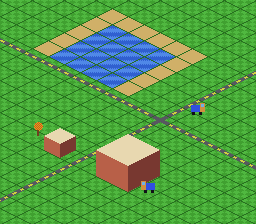
\includegraphics[width=0.75\textwidth]{figures/iso-sprite-demo.png}
	\caption{Two Lorries and a Tree over the Mode 2 Demonstration Scene}
	\label{fig:sprite-demo}
\end{figure}

\section{Programming Sprites}

\begin{enumerate}
	\item Write the sprite tile data into video memory, at the address that will be written to \texttt{STILES}.
	\item Write \texttt{STILES}, and the sprite tile size bits of the \texttt{TILESIZE} register.
	\item Write the table: entry $n$ is the words at offsets \texttt{0x7000} $+ 2n$ and \texttt{0x7001} $+ 2n$. Set the layer
	      field of every unused entry to 3.
	\item Make sure the sprite layers in use are not disabled in the Base Configuration register.
	\item Each frame, during vertical blanking, rewrite the \texttt{X} and \texttt{Y} fields of the sprites that moved.
\end{enumerate}

\section{Notes}

\begin{itemize}
	\item Scanning the 128 entries needs one read of the table per entry, at most 128 of the 512 PPU cycles of a line, from
	      internal memory.
	\item Sprites are not clipped to a window, and there is no priority bit per sprite beyond the layer.
\end{itemize}
